% SLAM Pipeline IPC & Thread Architecture
\documentclass[tikz, border=10pt]{standalone}
\usetikzlibrary{shapes.geometric, arrows.meta, positioning, calc}

\begin{document}

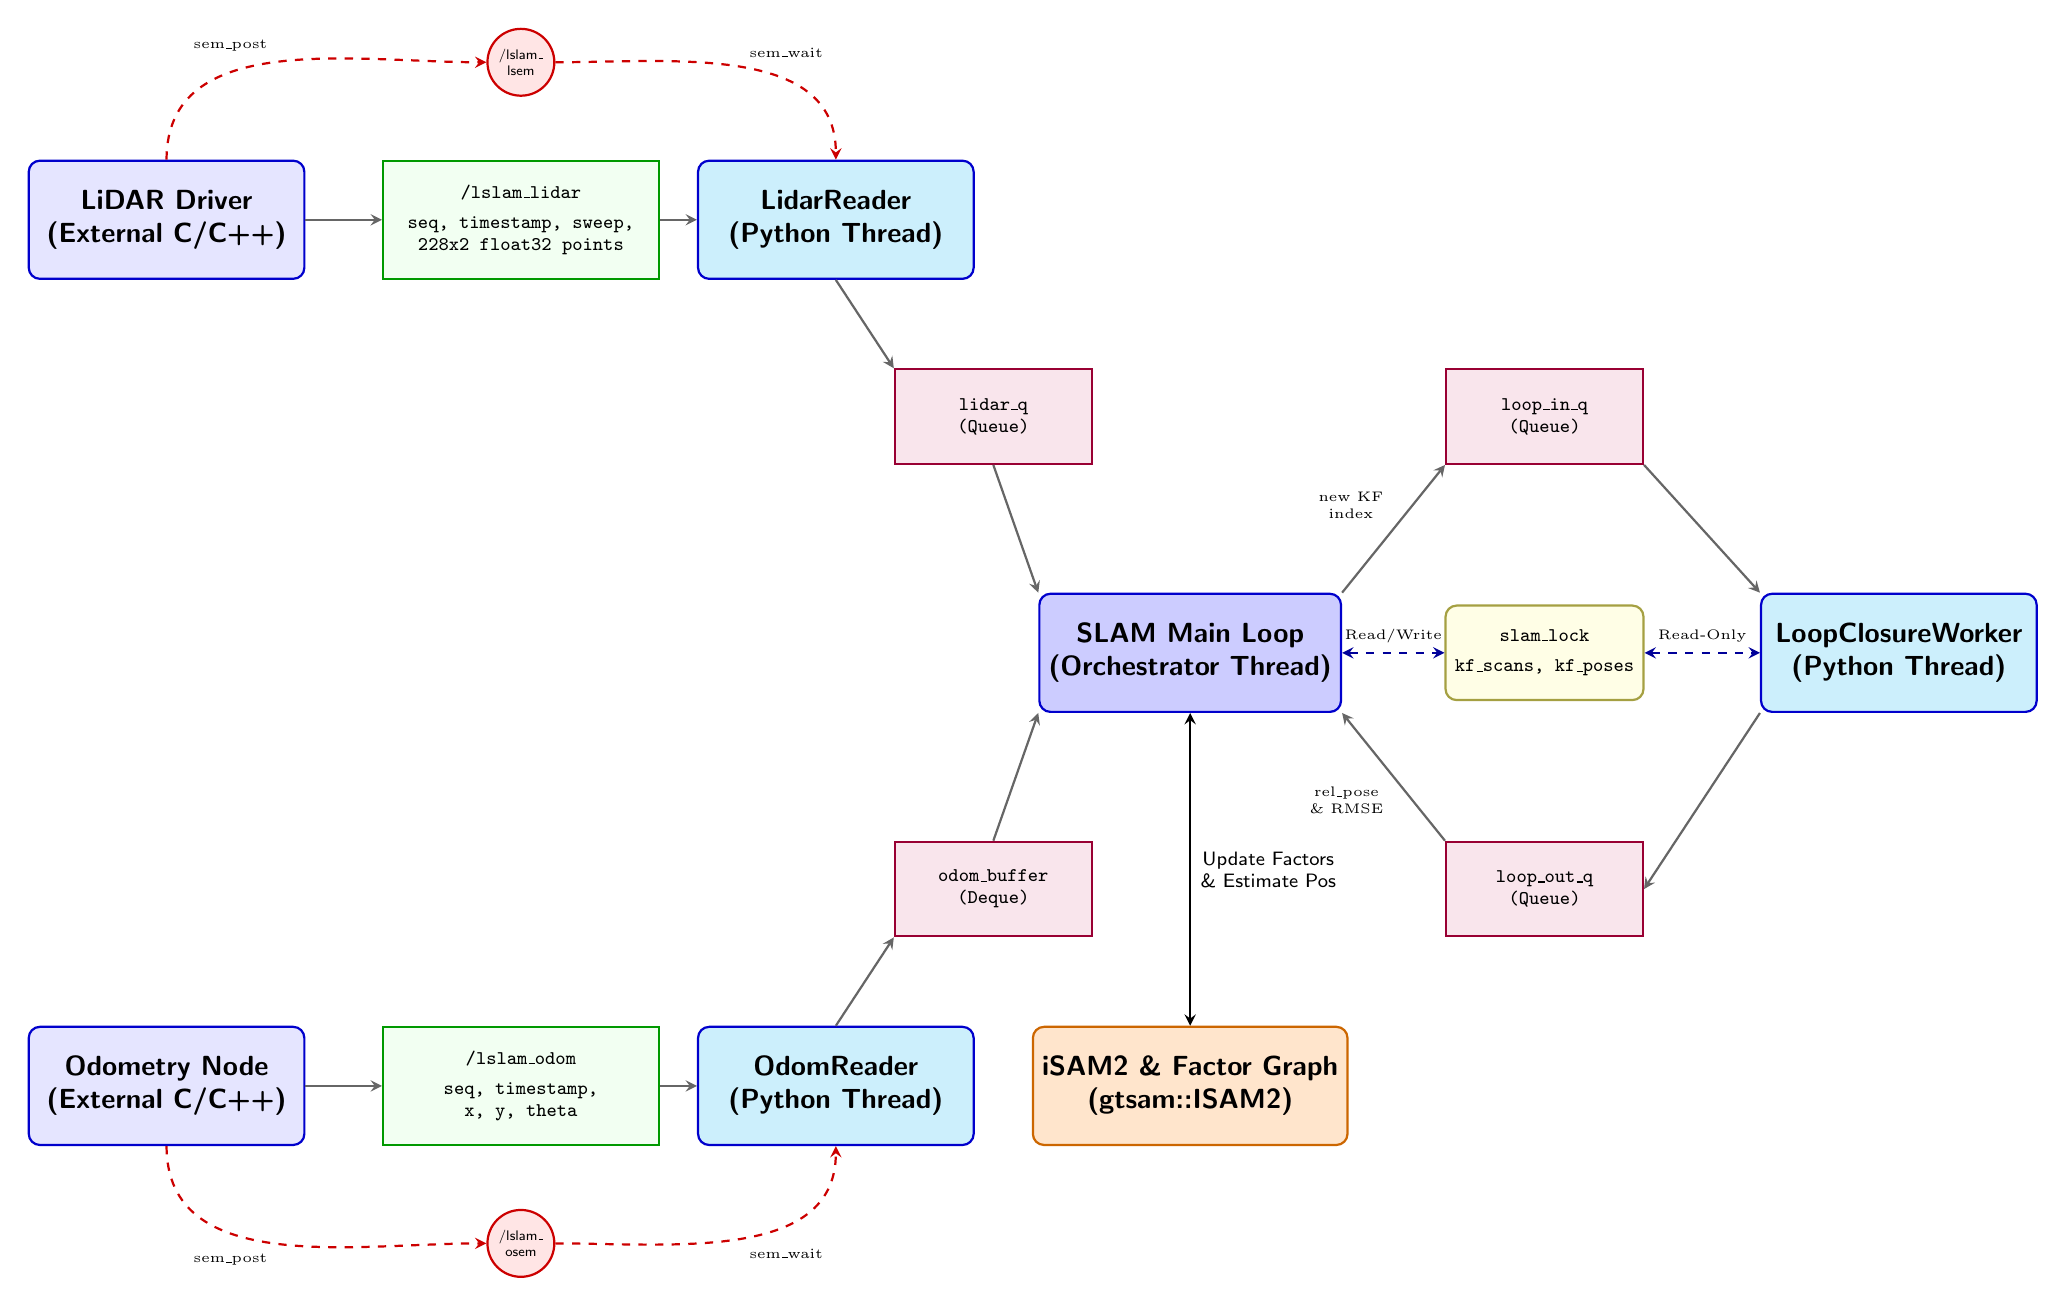
\begin{tikzpicture}[
    >=stealth,
    process/.style={rectangle, rounded corners, draw=blue!80!black, thick, fill=blue!10, minimum width=3.5cm, minimum height=1.5cm, align=center, font=\sffamily\bfseries},
    shm/.style={rectangle, draw=green!60!black, thick, fill=green!5, minimum width=3.5cm, minimum height=1.5cm, align=center, font=\ttfamily\scriptsize},
    queue/.style={rectangle, draw=purple!80!black, thick, fill=purple!10, minimum width=2.5cm, minimum height=1.2cm, align=center, font=\ttfamily\scriptsize},
    data/.style={rectangle, rounded corners, draw=yellow!60!black, thick, fill=yellow!10, minimum width=2.5cm, minimum height=1.2cm, align=center, font=\ttfamily\scriptsize},
    sem/.style={circle, draw=red!80!black, thick, fill=red!10, inner sep=2pt, align=center, font=\sffamily\tiny},
    arrow/.style={->, thick, draw=gray!80!black},
    signal/.style={->, dashed, thick, draw=red!80!black}
]

% ==================== Main Orchestrator ====================
\node[process, fill=blue!20] (Main) at (0, 0) {SLAM Main Loop\\(Orchestrator Thread)};

% ==================== LiDAR Pipeline (Top Left) ====================
\node[process] (ExtLidar) at (-13, 5.5) {LiDAR Driver\\(External C/C++)};

\node[shm] (shm_lidar) at (-8.5, 5.5) {/lslam\_lidar\\[1ex] seq, timestamp, sweep,\\ 228x2 float32 points};
\node[sem] (sem_lidar) at (-8.5, 7.5) {/lslam\_\\lsem};

\node[process, fill=cyan!20] (LidarReader) at (-4.5, 5.5) {LidarReader\\(Python Thread)};
\node[queue] (lidar_q) at (-2.5, 3.0) {lidar\_q\\(Queue)};

% LiDAR Connections
\draw[arrow] (ExtLidar.east) -- (shm_lidar.west);
\draw[signal] (ExtLidar.north) to[out=90, in=180] node[midway, above left, font=\tiny] {sem\_post} (sem_lidar.west);
\draw[arrow] (shm_lidar.east) -- (LidarReader.west);
\draw[signal] (sem_lidar.east) to[out=0, in=90] node[midway, above right, font=\tiny] {sem\_wait} (LidarReader.north);
\draw[arrow] (LidarReader.south) -- (lidar_q.north west);
\draw[arrow] (lidar_q.south) -- (Main.north west);


% ==================== Odometry Pipeline (Bottom Left) ====================
\node[process] (ExtOdom) at (-13, -5.5) {Odometry Node\\(External C/C++)};

\node[shm] (shm_odom) at (-8.5, -5.5) {/lslam\_odom\\[1ex] seq, timestamp,\\ x, y, theta};
\node[sem] (sem_odom) at (-8.5, -7.5) {/lslam\_\\osem};

\node[process, fill=cyan!20] (OdomReader) at (-4.5, -5.5) {OdomReader\\(Python Thread)};
\node[queue] (odom_buf) at (-2.5, -3.0) {odom\_buffer\\(Deque)};

% Odom Connections
\draw[arrow] (ExtOdom.east) -- (shm_odom.west);
\draw[signal] (ExtOdom.south) to[out=-90, in=180] node[midway, below left, font=\tiny] {sem\_post} (sem_odom.west);
\draw[arrow] (shm_odom.east) -- (OdomReader.west);
\draw[signal] (sem_odom.east) to[out=0, in=-90] node[midway, below right, font=\tiny] {sem\_wait} (OdomReader.south);
\draw[arrow] (OdomReader.north) -- (odom_buf.south west);
\draw[arrow] (odom_buf.north) -- (Main.south west);


% ==================== Loop Closure Pipeline (Right) ====================
\node[data] (SlamLock) at (4.5, 0) {slam\_lock\\[1ex] kf\_scans, kf\_poses};

\node[queue] (loop_in_q) at (4.5, 3.0) {loop\_in\_q\\(Queue)};
\node[queue] (loop_out_q) at (4.5, -3.0) {loop\_out\_q\\(Queue)};

\node[process, fill=cyan!20] (LoopWorker) at (9, 0) {LoopClosureWorker\\(Python Thread)};

% Loop Closure Connections
\draw[arrow] (Main.north east) -- (loop_in_q.south west) node[midway, above left, font=\tiny, align=center] {new KF\\index};
\draw[arrow] (loop_in_q.south east) -- (LoopWorker.north west);

\draw[arrow] (LoopWorker.south west) -- (loop_out_q.east);
\draw[arrow] (loop_out_q.north west) -- (Main.south east) node[midway, below left, font=\tiny, align=center] {rel\_pose\\\& RMSE};

% Shared State Connections
\draw[<->, dashed, thick, draw=blue!60!black] (Main.east) -- (SlamLock.west) node[midway, above, font=\tiny] {Read/Write};
\draw[<->, dashed, thick, draw=blue!60!black] (SlamLock.east) -- (LoopWorker.west) node[midway, above, font=\tiny] {Read-Only};


% ==================== GTSAM Backend (Bottom) ====================
\node[process, fill=orange!20, draw=orange!80!black] (ISAM) at (0, -5.5) {iSAM2 \& Factor Graph\\(gtsam::ISAM2)};

% Backend Connections
\draw[<->, thick, draw=black] (Main.south) -- (ISAM.north) node[midway, right, font=\sffamily\scriptsize, align=center] {Update Factors\\\& Estimate Pos};

\end{tikzpicture}

\end{document}